\documentclass[10pt]{scrarticle}
\usepackage{amsmath,amssymb,amsfonts}
\usepackage[english]{babel}
\usepackage{url}
\usepackage{graphicx}
\usepackage{caption}
\usepackage{subcaption}
\usepackage[left=2.5cm, right=2.5cm, top=2.5cm, bottom=2.5cm]{geometry}
\usepackage{setspace}
\usepackage[hidelinks]{hyperref}
\usepackage{enumitem}

\usepackage[backend=biber,
hyperref=true,
]{biblatex}
\addbibresource{references.bib}
\ExecuteBibliographyOptions{maxcitenames=1,mincitenames=1}

\setlist[itemize]{noitemsep}
\onehalfspacing

\begin{document}

\setstretch{1.3}
\begin{titlepage}
	\thispagestyle{empty}
	\centering

	\begin{minipage}[t]{\textwidth}
	
		\centering
		\Large{\uppercase{Project report}}
	
		\vspace{2cm}
	
		\rule{\textwidth}{1pt}
	
		\vspace{0.5cm}
	
		\textbf{\huge{Segmentation of Chronic Wounds}}
	
		\rule{\textwidth}{1pt}
	
		\vspace{5cm}
	\end{minipage}
	
	\begin{minipage}[t]{0.8\textwidth}
		\centering
	
		\large{\textbf{Cay Rahn}}
	
		\large{6255648}

		\vspace{3cm}
	
		\large{
			\noindent\begin{tabular}{@{}ll}
			\textbf{Course}:& KEN4244 Deep Learning for Image \& Video Processing\\
			\textbf{Academic Year}:& 2023/24
			\end{tabular}
		}
		
		\vspace{4cm}
		\large{\today}
	\end{minipage}
	
	
\end{titlepage}
\clearpage

\section{Introduction}

\subsection{Motivation}

\begin{itemize}
	\item Why is automatic Wound Segmentation so important? And why is it a complex problem?
	\item Manual segmentation by experts very time consuming
	\item experts differ in their segmentation
	\item changing lighting conditions, distance to camera, different cameras have impact on result
	\item controlled environment not feasible in clinical setting
	\item ideally, we want to be able to take pictures with a smartphone without overly complicated instructions for the person taking the picture
	\item experience as photographer should not be required, clinical proffessionals should be able to take pictures that are then segmented correctly
\end{itemize}


\subsection{Research Questions}

\begin{itemize}
	\item can the results be reproduced?
	\item what influence does the input image size have? Can we rescale the images and are able to transfer what is learned
	\item how robust is the model/architectures to transformations/distortions on the input
	\item XAI
\end{itemize}
\section{Dataset}

\begin{itemize}
	\item not many medical datasets on chronic wounds publicly available \cite{Oota_2023_WACV}
	\item often focus on specific type of chronic wounds - TODO: which one was over-represented again?
	\item used dataset consists of 2686 wound images with their corresponding masks introduced by \citeauthor{Oota_2023_WACV} \cite{Oota_2023_WACV}.
	\item 8 different wound types represented in dataset: venous ulcer, trauma wound, diabetic ulcer, surgical wound, arterial ulcer, cellulitis, pressure ulcer and a not further specified group of other wounds
	\item unfortunately, the wound classification is not available
\end{itemize}
\section{State of the Art}

\subsection{Semantic Segmentation}\label{sec:semantic-segmentation}

The segmentation of wounds belongs to the class of semantic segmentation problems, where a pixel-wise classification is performed. In the case of wound segmentation, there are two classes: foreground, which is the wound, and background. Deep Learning methods have become dominant in the last few years because they have become more accessible. Fully Convolutional Neural Networks (fCNN) as a starting point in research had the drawback of resulting in a low output resolution, and multiple techniques were invented to increase the output resolution \cite{Litjens2017}. This results in an encoder-decoder architecture as the base for the networks, inspired by auto-encoders \cite{LinkNet}, where the encoder subsamples and the decoder upsamples \cite{Norelyaqine2023}. In such architectures, the encoder generates context information, information in the feature space, while the decoder maps this information into the spatial context.

Pre-training for such models requires a vast amount of data. The typical object classification data set for such pre-training is the ImageNet data set \cite{SegNet}.

This project uses four segmentation models:: U-Net, LinkNet, FPN and PSPNet. All are improved architectures about a basic fCNN. Each architecture is described in detail to understand the challenges and approaches to localising information in space.

\paragraph{U-Net}

U-Net is a convolutional network developed for biomedical image segmentation based on an encoder-decoder architecture. Encoder and decoder are called contracting and expansive paths in the original paper, describing their function. They are also described as context and spatial paths \cite{MO2022626}. Both the encoder and decoder consist of different steps to encode and decode the image on different spatial levels. The encoder is a classical CNN; each step consists of two convolutions and a max pooling operation for downsampling. The decoder step upsamples the feature map followed by a convolution. The result is then concatenated with the corresponding feature map from the encoder path, and convolution is applied again. In the final layer, 1x1 convolution maps the feature vector to the desired number of classes. This architecture is visualised in Figure \ref{fig:unet-architecture}. \cite{unet}

\begin{figure}[htb!]
	\centering
	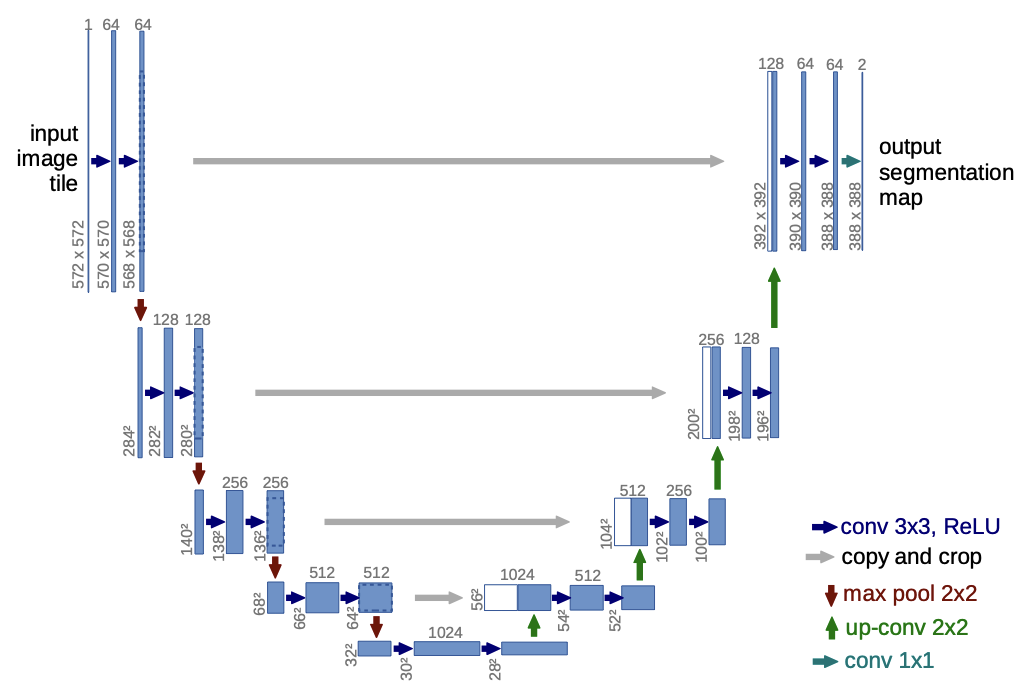
\includegraphics[width=0.8\textwidth]{fig/unet-architecture.png}
	\caption{U-Net architecture for 32x32 pixels in the lowes resolution. Blue boxes are feature maps with the number of feature-channels on top of the boxes and the size shown on the left size. Operations are indicated by the arrows. The skip connections are a concatenation. The figure originally create by \citeauthor{unet} \cite{unet}.}
	\label{fig:unet-architecture}
\end{figure}

The skip connections, connecting the different levels of encoder and decoder prevent a loss of information and extract the features at different resolutions to retrieve spatial information. By doing this, it is one of the first architectures to improve the classical fCNN for semantic segmentation \cite{Litjens2017}. While U-Net provides spatial localisation of features, its ability to generalise to multi-scale information is limited \cite{Norelyaqine2023}.

One restriction is that the input size must be chosen to apply all 2x2 max-pooling operations in the encoder to an even x and y size.


\paragraph{LinkNet}

Like U-Net, LinkNet consists of an encoder block for downsampling and a decoder block for upsampling. The downsampling is not done by max pooling as in the U-Net architecture but by using a stride of 2 in a convolutional layer. The initial encoder block also differs from the following blocks as it uses a larger kernel and max pooling. The decoder blocks upsample by a factor of 2 in each block. The final block differs again from the previous blocks. The main difference to the U-Net architecture is how the skip connections are used: Similarly to the U-Net, there are skip connections between the corresponding steps of the encoder and decoder, but the feature map from the encoder is not concatenated but added to decoder data. The LinkNet architecture is visualised in Figure \ref{fig:LinkNet-architecture}. \cite{LinkNet}

\begin{figure}[htb!]
	\centering
	\includegraphics[width=0.5\textwidth]{fig/LinkNet-architecture.png}
	\caption{A visualisation of the LinkNet architecture originally provided by \citeauthor{SegmentationModels} \cite{SegmentationModels}.}
	\label{fig:LinkNet-architecture}
\end{figure}


%\begin{itemize}
%	\item "LinkNet sends spatial information directly from the encoder to the matching decoder, conserving as much of the image’s spatial information as feasible."
%	\item "directly connects shallow feature map in encoder module to the decoder module of the corresponding size" $\rightarrow$ accurate position information on shallow layer, avoids redundant parameters and computations \cite{Norelyaqine2023}
%\end{itemize}

The implementation used in this project has four skip connections instead of the original three \cite{SegmentationModels}. Similarly to the U-Net, the input size is restricted, so that every upsampling operation can be applied to an even x and y size.

LinkNet has been shown to achieve better results than U-Net under similar conditions \cite{Gao2022}.

\paragraph{FPN}

The Feature Pyramid Network (FPN) architecture creates feature maps of various sizes in multiple layers \cite{Norelyaqine2023}. Like the other architectures, it consists of an encoder and a decoder, called bottom-up and top-down pathways here\cite{fpn}. Similarly to U-Net, feature maps at different scales with a scaling step of 2 are created in the encoder \cite{fpn}. In the decoder, the feature maps are upsampled and combined with the encoder information of the same level. Similarly to LinkNet, addition is used in the skip connections, but a 1x1 convolution is applied. By doing this, so-called feature pyramids are built, containing features at different resolutions. \citeauthor{kirillov2019panoptic} proposed using these feature pyramids to obtain a segmentation by merging the feature maps using addition or concatenation \cite{kirillov2019panoptic, SegmentationModels}. The architecture is visualised in Figure \ref{fig:fpn-architecture}.

\begin{figure}[htb!]
	\centering
	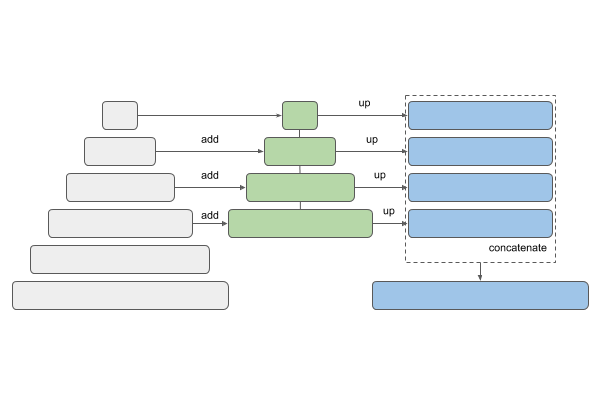
\includegraphics[width=0.6\textwidth]{fig/fpn-architecture.png}
	\caption{A visualisation of the FPN architecture originally provided by \citeauthor{SegmentationModels} \cite{SegmentationModels}. Note, that the feature maps can combined either by concatenation or addition.}
	\label{fig:fpn-architecture}
\end{figure}


\paragraph{PSPNet}

The central part of the Pyramid Scene Parsing Network (PSPNet) is the pyramid pooling module, visualised in part c of Figure \ref{fig:pspnet-architecture}, which extracts context information at different scales. A feature map extracted with a pre-trained backbone is pooled at different pyramid scales. This means that global pooling and sub-regions on different locations are used to extract features from a global to a more fine-grained scale. Each of those scales is passed through a 1x1 convolution and afterwards upsampled to the size of the original feature map. All feature maps, including the original feature map from the backbone, are concatenated and used to extract the final prediction. By this, features on different scales are combined. \cite{Zhao2017, ArcGIS}

\begin{figure}[htb!]
	\centering
	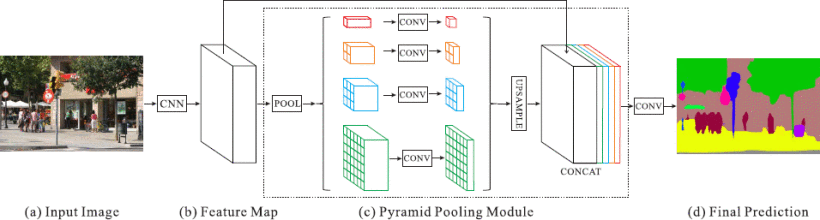
\includegraphics[width=\textwidth]{fig/pspnet-architecture.png}
	\caption{Visualization of the PSPNet-architecture. Originally created by \citeauthor{Zhao2017} \cite{Zhao2017}.}
	\label{fig:pspnet-architecture}
\end{figure}

\subsubsection{Optimisation and Evaluation}

Several methods exist to evaluate how good a predicted segmentation is. Since semantic segmentation performs a pixel-wise classification, resulting in a segmentation mask, classical metrics such as accuracy and precision are available. Two performance metrics commonly used in semantic segmentation in medical imaging are the Dice Coefficient and the Intersection over Union (IoU) score. They indicate the segmentation quality better than pixel-wise accuracy \cite{Eelbode}.

\paragraph{IoU-Score}

The IoU-Score (Intersection over Union), also known as the Jaccard index $J$, describes the ratio between the intersection of the ground truth mask $y$ and the predicted mask $\tilde{y}$ and the union of the predicted and the ground truth mask. This compares the similarity of the two masks \cite{Cho2021WeightedIO}.

\begin{align}
	\text{IoU}(y, \tilde{y} :&= \frac{\text{Area of overlap}}{\text{Area of union}}\\
	&=\frac{|y \cap \tilde{y}|}{|y \cup \tilde {y}|}
\end{align}


\paragraph{Dice Coefficient}

The Dice coefficient is the F1 score calculated for the image masks. Regarding intersection and union, it calculates the ratio between two times the overlap between ground truth $y$ and predicted mask $\tilde{y}$ and the total area.

\begin{align}
	\text{Dice}(y, \tilde{y}) :&= 2 \cdot \frac{\text{Area of overlap}}{\text{Total area}}\\
	&= 2 \cdot \frac{|y \cap \tilde{y}|}{|y| + |\tilde{y}|}
\end{align}

To gain more insight into the type of errors the model makes, the rate of false positives and false negatives can be reported and then used to differentiate Type I and Type II errors \cite{DFUC2022}.

% "The difference between the two metrics is that the IoU penalizes under- and over-segmentation more than DSC"

\paragraph{Loss function}

Although the Dice Coefficient and IOU-Score are the most commonly used evaluation metrics, pixel-wise cross-entropy is often used as a loss function \cite{Eelbode}. Since it is shown that there is no direct link between pixel-wise cross-entropy, either weighted or not, and Dice Coefficient and IoU-Score, this choice does not make sense because it does not optimise towards the goal.

Differentiable approximations for Dice Coefficient and IoU-Score exist that can be used to perform more goal-orientated optimisation. Both metrics and loss functions are shown to be linked to each other \cite{Eelbode}.

% DiceLoss is used in the code

\subsubsection{Data Augmentation}

Data Augmentation is a valuable technique to make trained models more robust and accurate. This is especially true if available data is limited, as the data set size can be increased or the data set can be made more diverse.

For images, there exist several different possible augmentations. First, there are different positional augmentations, including cropping, flipping, rotating and resizing the image. Another class of augmentations is colour augmentation, which changes the image's brightness, contrast or saturation. Other augmentations include blurring and dropouts.

Not every augmentation is appropriate for every application. Rotating images of standing animals by 180 degrees, for example, would not make sense, while the rotation of wound images is appropriate. Therefore, augmentations must be chosen carefully depending on the application.


% https://nanonets.com/blog/data-augmentation-how-to-use-deep-learning-when-you-have-limited-data-part-2/
% https://www.v7labs.com/blog/data-augmentation-guide


\subsection{Wound Segmentation}


As already discussed in the motivation of this project, wound segmentation is a complex problem due to wound characteristics such as different tissues and, therefore, edges inside of a wound itself on one side and technical reasons such as, e.g. varying lighting, distance to the wound and different angles. 

Before Deep Learning became easily accessible and popular, methods based on features describing colour and textures, region-growing with optimal thresholding algorithms, and classical machine learning models were used to perform segmentation \cite{Scebba2022}. Convolutional Neural Networks replaced manually extracted features with autonomously learned ones \cite{Scebba2022}. Some methods included pre-processing steps to remove the background by, e.g., user interaction indicating the background, using a standardized background when taking the image, or using manual feature engineering to detect the background more efficiently and make the wound segmentation task easier. Such non-automatic steps limit the use of the segmentation algorithms because they either require more resources in the image-taking process or the segmentation process or are specifically tailored for specific lighting conditions or camera settings.

The Diabetic Foot Ulcer Challenge 2022 used FCN, U-Net and SegNet with different backbones and categorical cross-entropy loss as the baseline for their challenge, indicating those methods reflect the current state of the art that needs to be improved \cite{DFUC2022}. Generally, such classic models are commonly used and extended with minor adaptions. Two methods stood out in the performed literature review, including more sophisticated adaptions.

\citeauthor{Scebba2022} proposed a method consisting of two steps: An object detection step that produces bounding boxes containing the wounds and a second step that performs segmentation on those areas. Segmentation is performed using classical architectures for semantic segmentation, as described in section \ref{sec:semantic-segmentation}. The loss function used was a pixel-wise weighted binary cross-entropy loss. Weighting was calculated based on the number of wound pixels and background pixels of each training set fold. Unfortunately, no code with more implementation details was available and the approach therefore not investigated in detail.

\citeauthor{Oota_2023_WACV} claim they set a new state of the art for wound segmentation while providing a data set together with their work \cite{Oota_2023_WACV}. The latter made them a suitable method for further investigation in this project's scope. Their approach is described in more detail in the following section.

\subsubsection{WSNet}

The framework proposed by \citeauthor{Oota_2023_WACV} uses the previously described segmentation architectures: U-Net, LinkNet, PSPNet, and FPN. Experiments with different backbones were performed in their work. However, in this project's scope, MobileNet \cite{howard2017mobilenets} is mainly used since it is the smallest one, which allows faster training, which is needed in the limited time of the project.

ImageNet pre-trained weights are used. WSNet also describes pre-training specific to wounds, called Wound-Domain Adaptive Pre-training. During this pre-training, wound images are classified into five different ulcer types.

\citeauthor{Oota_2023_WACV} experimented with data augmentation on the training data and the corresponding masks, including optical distortion, horizontal flip, random rotation, blur, and more, to make their models more robust.

\paragraph{Global-Local Architecture}

The network architecture proposed by \citeauthor{Oota_2023_WACV} is called Global-Local architecture. It consists of two segmentation models, a global model and a local model, combining the result for the final segmentation. The global model is a standard segmentation model of one of the four architectures described in section \ref{sec:semantic-segmentation}. In the global model, the image (size 192x192x3) is split into 16 non-overlapping patches, resulting in a size of 48x48x3 per patch. The patches are then stacked, resulting in a size of 48x48x(3x16). The patches are the input to 16 local models in parallel, with shared weights between the local models. The output is eventually combined to obtain a full-sized mask. This mask and the output of the global model are concatenated to a mask of size 192x192x2, and a final convolution of size 1x1 results in the predicted mask. This architecture is motivated by the need to combine global signals from the entire image and local signals from smaller patches for more details. Only capturing local signals might cause an incomplete segmentation for large wounds. \cite{Oota_2023_WACV}

Although the combination of global and local signals sounds reasonable initially, it is interesting that this approach is combined with segmentation models that already contain different context sizes and localisation in these context sizes, as described in section \ref{sec:semantic-segmentation}. An explicitly chosen patch size implies some property of the wound images that makes this size particularly important for local information. \citeauthor{Oota_2023_WACV} stated in their paper that they tested different patch sizes and chose 48 because it led to the best results \cite{Oota_2023_WACV}, supporting the theory that this patch size yields more information than others.


\paragraph{Reported Results}

\citeauthor{Oota_2023_WACV} report that wound-specific pre-training improves the resulting segmentation. Furthermore, they find that data augmentation leads to improvements. As expected, the local-only models perform significantly worse than using the segmentation model as intended in a global way. Furthermore, they find that combining global and local models leads to an improved performance compared to the global models. This indicates that the chosen patch size yields valuable information for the segmentation. The best results are therefore achieved with wound-specific pre-training, data augmentation and the invented Global-Local architecture.

\begin{table}[htb!]
	\centering
	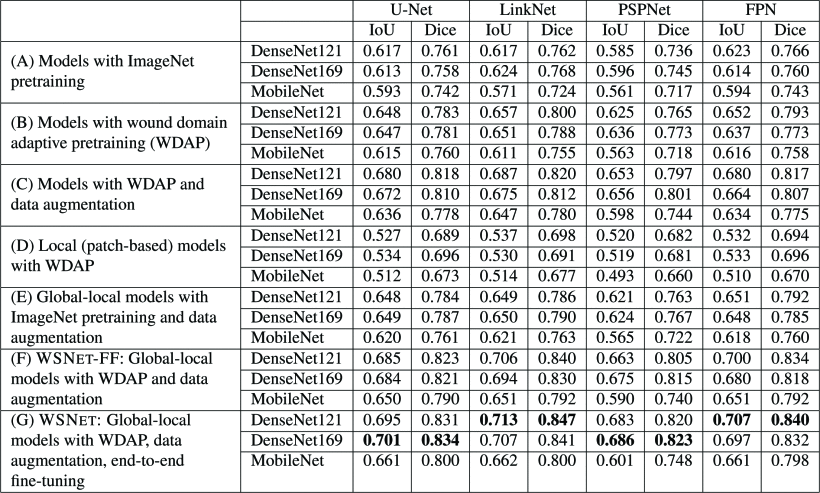
\includegraphics[width=0.9\textwidth]{fig/wsnet-results.png}
	\caption{Results reported by \citeauthor{Oota_2023_WACV} \cite{Oota_2023_WACV}.}
	\label{table:results-wsnet}
\end{table}

Reporting such results always leads to the question of whether they are reproducible. This is especially the case with the Global-Local architecture with a specific patch size, leading to questioning whether the patch size can be generalised to other image sizes and other data sets.




\section{Technical Information}

\subsection{Prior Experience}

I have a strong programming background, consisting of a B.Sc. in Computer Science and three years of work experience in Web Developement with Python. Beside the content of the course Advanced Concepts of Machine Learning, I have no prior experience with Deep Learning.

\subsection{Code and Data Availability}

The code produced in the scope of the project is available on GitHub: \url{https://github.com/Zianor/DLIV-chronic-wound-segmentation}. Package versions are included to ensure reproducability.

The used data is available on GitHub as well: \url{https://github.com/subbareddy248/WSNET/} \cite{Oota_2021_WACV, Oota_2023_WACV}. Availability on a later point of time cannot be guaranteed.

\subsection{Libraries}

Several libraries were used in this project. The Deep Learning framework all work is based on is Tensorflow with Keras \cite{tensorflow2015-whitepaper, chollet2015keras}. The implementation of the 4 used network architectures was provided by the Python library \texttt{segmentation\_models} \cite{SegmentationModels}. Image augmentations were performed with \texttt{Albumentations} \cite{albumentations}.

\subsection{Learning Process}

\begin{itemize}
	\item Getting familiar with tensorflow
	\item learning about the state of the art in segmantic segmentation and segmentation of wound images and evaluation methods
	\item more experience in dealing with paper results and how trustworthy they are
	\item first, I planned on spending more time on the results of the chosen paper and experimenting with different augmentations and explainability
	\item after doing research about segmentation models I got sceptical about the general approach and spend a lot of time in researching semantic segmentation and the how and why
	\item 
\end{itemize}


\subsection{Used Hardware}

All computations are performed on one of two different machines: a MacBook Air (24\,GB RAM, Apple M2 Chip with an 8-core GPU) or a computer with 16GB and a nvidia GeForce GTX 1070 Ti as GPU. The package versions for GPU-utilization on MacOS are included in the package versions on GitHub.



\printbibliography

\end{document}
